%!TEX root = ../report.tex

\begin{document}
    \chapter{Introduction}

Robots generate a large amount of data from different types of sensors attached to it and also from its hardware components. In our previous research work \cite{ravichandranworkbench}, we have conducted an extensive qualitative and quantitative analysis to find better databases and architectures that effectively store these data and consume it for further operations. Results from our previous work show that a single database is not suitable for every robotic scenario. For example, in terms of handling large BLOB data, MongoDB stored them faster but reading the data was slower compared to CouchDB \cite{ravichandranworkbench}. Also, to complete a given task robot depends on multiple sources of information from internal sensors, as well as external sources for example world model, kinematic model, etc.. 

Adoption of multiple databases for robotic applications requires a unique way of mediation to view multiple databases as a single federated database. Mediator approach helps to integrate data from different sources and produce an only result back to robots. Mediator abstracts the information of how data is being stored in various data sources from a robot and allows robotic applications stream data to mediator independent of databases used in the back-end.

To Map the data generated by robots with multiple databases, the mediator system requires a proper data model predefined in the context of robotic applications. Modeling robot produced data helps to generalize the structure of data and defining relations between different entities (e.g., tasks,  sensors, robots, location ) in a robotic application scenario. If we have a well defined robotic data models, then the mediator will get the ability to mutate or query data from different data sources. Also, it is essential that any robotic use-cases should be able to extend these data models.


As mentioned in these papers \cite{ahmed1991pegasus,fahl1993amos,arens1996query,chawathe1994tsimmis,chawathe1994tsimmis,shoens1993rufus}, mediators are being used to integrate data from different data sources, and few architectures support single data model (e.g., SQL), and others recommend for different data models (e.g., SQL, NoSQL, document store, etc..). Also, they differ from query languages, ease of implementation, components used in their architecture. This project mainly focuses on defining semantic based models for sensor data to make it more interoperable with other systems or even in multi-robot systems, and implementing a mediator system which acts as a middle-ware between robots and databases. 

    \section{Motivation}
    
Streamlining the data produced from different sensors in robotic applications is a tedious task, and there are no specific standards to organize the data in terms of making relations between the entities and also giving context to the data. It will be even more complicated when we have a multi-robot platform and sharing data between them, and backing up the data into a database for fault diagnosis.

Currently, in the ROPOD\footnote{ROPOD is a EU funded project to develop "Ultra-flat, ultra-flexible, and cost-effective robotic pods for handling legacy in logistics"} project, there is a single black box component has been developed to simulate the robot test cases. During the simulation black box stores the data produced by the sensors as dumps into a single MongoDB instance locally.  

The first problem here is since the sensor data stored as dumps which makes the consumer's\footnote{A consumer can be either humans or machines.} inability to make queries against the data. 

And the second problem is missing contexts and the entity-relationship model. For example, if a consumer tries to query the data from dumps, it will be unsure that which sensor produced this data from which robot/black-box at which location and time, and who triggered this test case. What we mean "missing context" is if humans read the data they will understand what's the meaning of each parameter, but if a different robot/black-box tries to consume the data produced by other robots, then the context about the data should be shared somewhere globally.

The final problem is, what if we have a situation where multi-robots tries to share data or human controller wants to do fault-diagnosis on data shared on multi-robots. 


These significant issues inspired us to find a suitable Entity-Relationship data model and unique mediation system to query heterogeneous sensor data from multiple data sources regardless of the database type.


    \section{Structure}
	
		\begin{itemize}
			\item Section x concisely describes the background knowledge of the topics which are relevant to this work.
		\end{itemize}
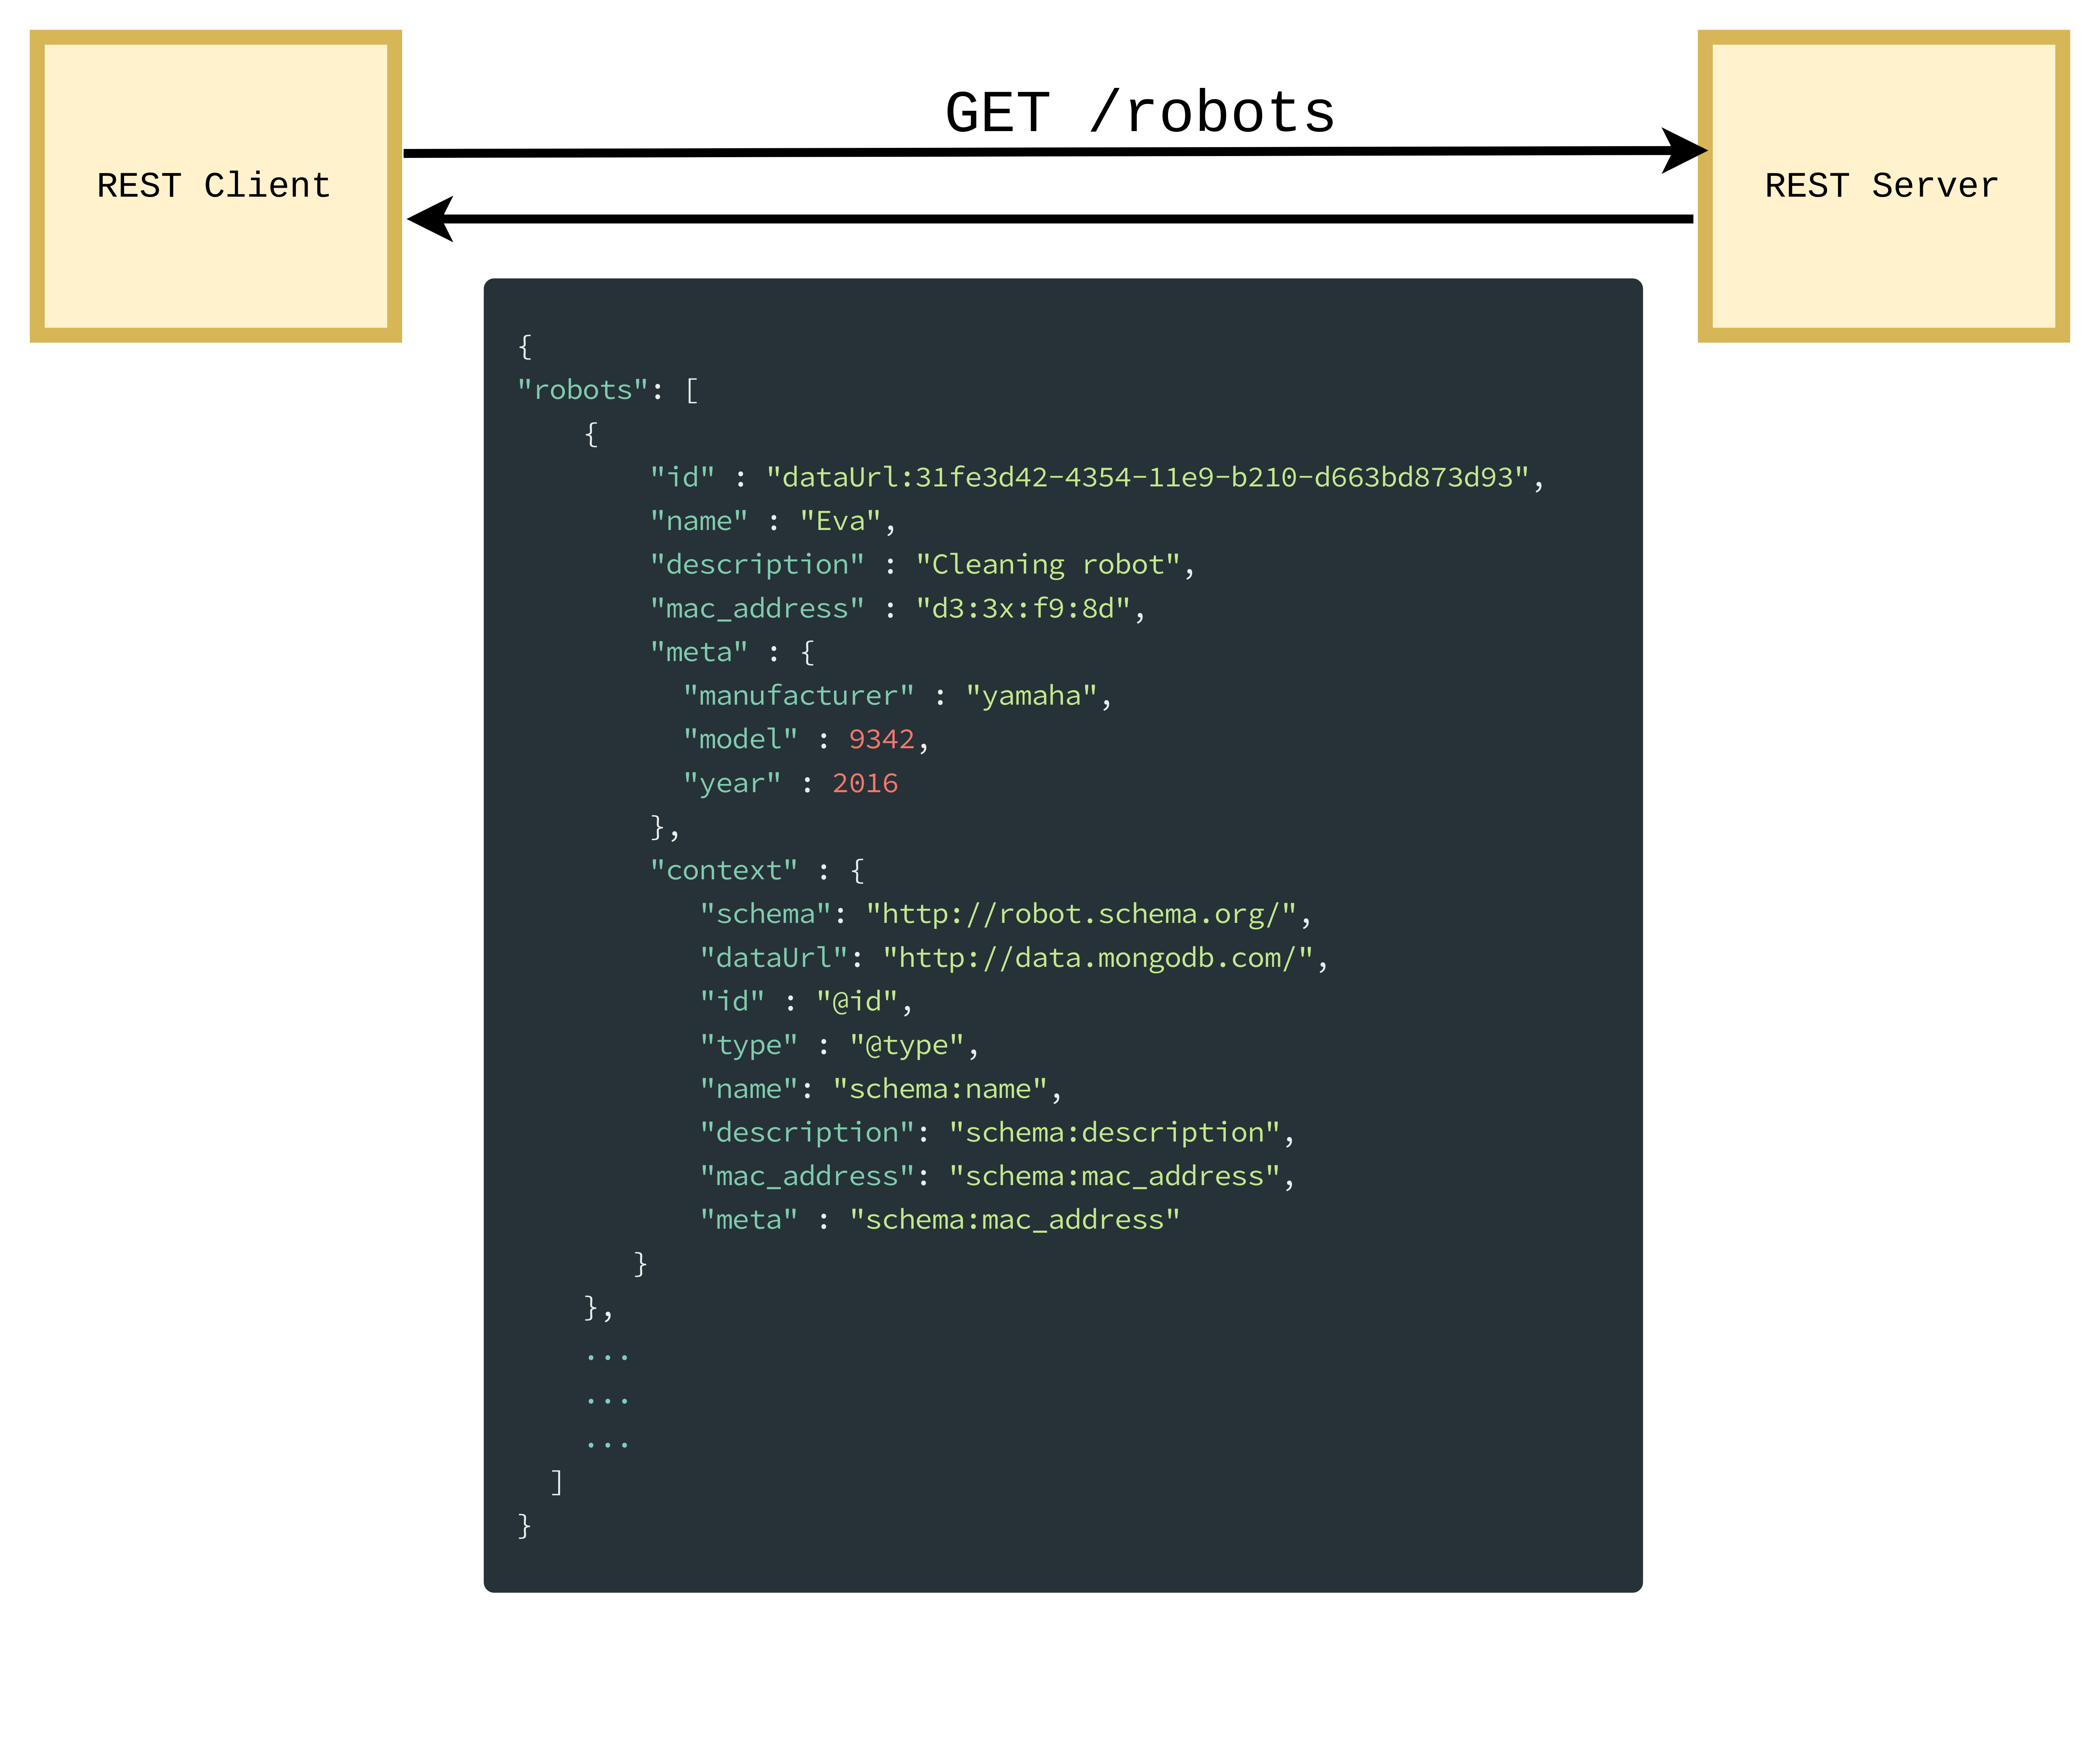
\includegraphics[scale=0.08]{image}

\let\cleardoublepage\clearpage
\end{document}
